\documentclass[tikz,border=4pt]{standalone}
\usepackage{amsmath}
\begin{document}
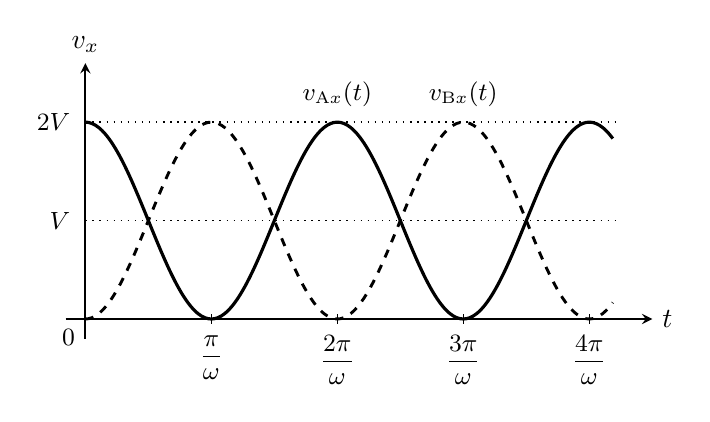
\begin{tikzpicture}[>=stealth, thick, scale=1.0]
  % Axes: x = t in units where pi/omega = 1.6 cm; y = v_x in units where V = 1.25 cm (2V = 2.5 cm)
  \draw[->, line width=0.65pt] (-0.25, 0) -- (7.2, 0) node[right] {$t$};
  \draw[->, line width=0.65pt] (0, -0.25) -- (0, 3.25) node[above] {$v_x$};
  \node[below left, font=\small] at (0, 0) {$0$};

  % Horizontal reference lines V and 2V
  \draw[dotted, line width=0.55pt] (0, 1.25) -- (6.8, 1.25);
  \draw[dotted, line width=0.55pt] (0, 2.50) -- (6.8, 2.50);
  \node[left, font=\small] at (-0.06, 1.25) {$V$};
  \node[left, font=\small] at (-0.06, 2.50) {$2V$};

  % v_Ax(t) = V (1 + cos(omega t)): solid
  \draw[line width=1.15pt, domain=0:6.7, samples=160, smooth]
    plot (\x, {1.25*(1 + cos(deg(pi*\x/1.6)))});

  % v_Bx(t) = V (1 - cos(omega t)): dashed
  \draw[dashed, line width=1.05pt, domain=0:6.7, samples=160, smooth]
    plot (\x, {1.25*(1 - cos(deg(pi*\x/1.6)))});

  % Ticks on t-axis
  \foreach \x/\lbl in {1.6/\dfrac{\pi}{\omega}, 3.2/\dfrac{2\pi}{\omega}, 4.8/\dfrac{3\pi}{\omega}, 6.4/\dfrac{4\pi}{\omega}} {
    \draw[line width=0.55pt] (\x, 0.06) -- (\x, -0.06);
    \node[below, font=\small] at (\x, -0.08) {$\lbl$};
  }

  % Curve labels
  \node[above, font=\small] at (3.2, 2.56) {$v_{\mathrm{A}x}(t)$};
  \node[above, font=\small] at (4.8, 2.56) {$v_{\mathrm{B}x}(t)$};
\end{tikzpicture}
\end{document}
